\documentclass[12pt,a4paper]{article}
\usepackage{geometry}
\usepackage{slashbox}
\geometry{
	a4paper,
	total={170mm,257mm},
	left=20mm,
	right=20mm,
	top=20mm,
	bottom=20mm
}
\usepackage{graphicx}
\usepackage{pdfpages}
\usepackage{placeins}
\usepackage{float}

\usepackage{polski}
\usepackage[utf8]{inputenc}

\begin{document}
	
	\begin{titlepage}
		\newgeometry{top=5.5cm, bottom=3cm}
		
		\centering
		{\huge\bfseries Logika układów cyfrowych lab.\par}
		
		\vspace{0.5cm}
		Prowadzący: Mgr inż. Antoni Sterna (E02-38m, wtorek 17:05) \\
	
		\vspace{1.1cm}
		{\Large sprawozdanie 4 - 2017.11.07\par}
		\vfill
		
		{\large\bfseries Jakub Dorda 235013\par}
		{\large\bfseries Marcin Kotas 235098\par}
		
		\vspace{1cm}
		\today \\ \LaTeX
		
		\restoregeometry
	\end{titlepage}

	\section{Wprowadzenie/cel ćwiczeń}
		
		
	\section{Subtraktor szeregowy}
	
		\subsection{Graf:}
		
			
	\section{Komparator szeregowy}
	
		\subsection{Graf:}
		
	
		\subsection{Tabela prawdy i tablice Karnaugh:}
			\begin{table}[H]
			\begin{minipage}{.5\textwidth}
				\caption{Tabela Prawdy - funkcja przejść}
				\vspace{0.2cm}
				\centering
				\begin{tabular}{cccc|cc}
					\multicolumn{4}{c|}{\(t\)}	&	\multicolumn{2}{c}{\(t+1\)} \\
					\(q_1\)&\(q_0\)&\(z_1\)&\(z_0\)&\(q_1\)&\(q_0\)\\\hline
					0	&	0	&	0	&	0	&	-	&	-	\\
					0	&	0	&	0	&	1	&	-	&	-	\\
					0	&	0	&	1	&	0	&	-	&	-	\\
					0	&	0	&	1	&	1	&	-	&	-	\\\hline
					0	&	1	&	0	&	0	&	0	&	1	\\
					0	&	1	&	0	&	1	&	0	&	1	\\
					0	&	1	&	1	&	0	&	1	&	0	\\
					0	&	1	&	1	&	1	&	0	&	1	\\\hline
					1	&	0	&	0	&	0	&	1	&	0	\\
					1	&	0	&	0	&	1	&	0	&	1	\\
					1	&	0	&	1	&	0	&	1	&	0	\\
					1	&	0	&	1	&	1	&	1	&	0	\\\hline
					1	&	1	&	0	&	0	&	1	&	1	\\
					1	&	1	&	0	&	1	&	0	&	1	\\
					1	&	1	&	1	&	0	&	1	&	0	\\
					1	&	1	&	1	&	1	&	1	&	1	\\
				\end{tabular}
			\end{minipage}%
			\begin{minipage}{.5\textwidth}
				\caption{Tablica Karnaugh dla $q_1$}
				\vspace{0.2cm}
				\centering
				\begin{tabular}{c|c|c|c|c}
					\backslashbox{$z_1z_0$}{$q_1q_0$}&00&01&11&10\\\hline
					00	&	-	&	0	&	1	&	1	\\\hline
					01	&	-	&	0	&	0	&	0	\\\hline
					11	&	-	&	0	&	1	&	1	\\\hline
					10	&	-	&	1	&	1	&	1	
				\end{tabular}
				\vspace{1cm}
				
				\caption{Tablica Karnaugh dla $q_0$}
				\vspace{0.2cm}
				\centering
				\begin{tabular}{c|c|c|c|c}
					\backslashbox{$z_1z_0$}{$q_1q_0$}&00&01&11&10\\\hline
					00	&	-	&	1	&	1	&	0	\\\hline
					01	&	-	&	1	&	1	&	1	\\\hline
					11	&	-	&	1	&	1	&	0	\\\hline
					10	&	-	&	0	&	0	&	0	
				\end{tabular}
			\end{minipage}
			\end{table}
		
			\begin{table}[H]
			\begin{minipage}{.5\textwidth}
				\caption{Tabela Prawdy - funkcja wyjść}
				\vspace{0.2cm}
				\centering
				\begin{tabular}{cccc|cc}
					\(q_1\)&\(q_0\)&\(z_1\)&\(z_0\)&\(y_1\)&\(y_0\)\\\hline
					0	&	0	&	0	&	0	&	-	&	-	\\
					0	&	0	&	0	&	1	&	-	&	-	\\
					0	&	0	&	1	&	0	&	-	&	-	\\
					0	&	0	&	1	&	1	&	-	&	-	\\\hline
					0	&	1	&	0	&	0	&	0	&	1	\\
					0	&	1	&	0	&	1	&	0	&	1	\\
					0	&	1	&	1	&	0	&	1	&	0	\\
					0	&	1	&	1	&	1	&	0	&	1	\\\hline
					1	&	0	&	0	&	0	&	1	&	0	\\
					1	&	0	&	0	&	1	&	0	&	1	\\
					1	&	0	&	1	&	0	&	1	&	0	\\
					1	&	0	&	1	&	1	&	1	&	0	\\\hline
					1	&	1	&	0	&	0	&	1	&	1	\\
					1	&	1	&	0	&	1	&	0	&	1	\\
					1	&	1	&	1	&	0	&	1	&	0	\\
					1	&	1	&	1	&	1	&	1	&	1	\\
				\end{tabular}
			\end{minipage}%
			\begin{minipage}{.5\textwidth}
				\caption{Tablica Karnaugh dla $y_1$}
				\vspace{0.2cm}
				\centering
				\begin{tabular}{c|c|c|c|c}
					\backslashbox{$z_1z_0$}{$q_1q_0$}&00&01&11&10\\\hline
					00	&	-	&	0	&	1	&	1	\\\hline
					01	&	-	&	0	&	0	&	0	\\\hline
					11	&	-	&	0	&	1	&	1	\\\hline
					10	&	-	&	1	&	1	&	1	
				\end{tabular}
				\vspace{1cm}
				
				\caption{Tablica Karnaugh dla $y_0$}
				\vspace{0.2cm}
				\centering
				\begin{tabular}{c|c|c|c|c}
					\backslashbox{$z_1z_0$}{$q_1q_0$}&00&01&11&10\\\hline
					00	&	-	&	1	&	1	&	0	\\\hline
					01	&	-	&	1	&	1	&	1	\\\hline
					11	&	-	&	1	&	1	&	0	\\\hline
					10	&	-	&	0	&	0	&	0	
				\end{tabular}
			\end{minipage}
			\end{table}
		
		\subsection{Minimalizacje:}
			\begin{displaymath}
			q_1(t+1) = y_1 = z_1\bar{z_0} + q_1z_1 + q_1\bar{z_0}= \overline{\overline{z_1\bar{z_0}} \cdot \overline{q_1z_1} \cdot \overline{q_1\bar{z_0}}}
			\end{displaymath}
			\begin{displaymath}
			q_0(t+1) = y_0 = \bar{z_1}z_0 + q_0\bar{z_1} + q_0z_0= \overline{\overline{\bar{z_1}z_0} \cdot \overline{q_0\bar{z_1}} \cdot \overline{q_0z_0}}
			\end{displaymath}
		
		\subsection{Użyte wzory:}
			\begin{equation}
			\overline{a+b}=\bar{a}\cdot\bar{b}
			\end{equation}
		
		\subsection{Schemat układu:}
		
		\vspace{1.5cm}
		\begin{center}
			\makebox[\textwidth]{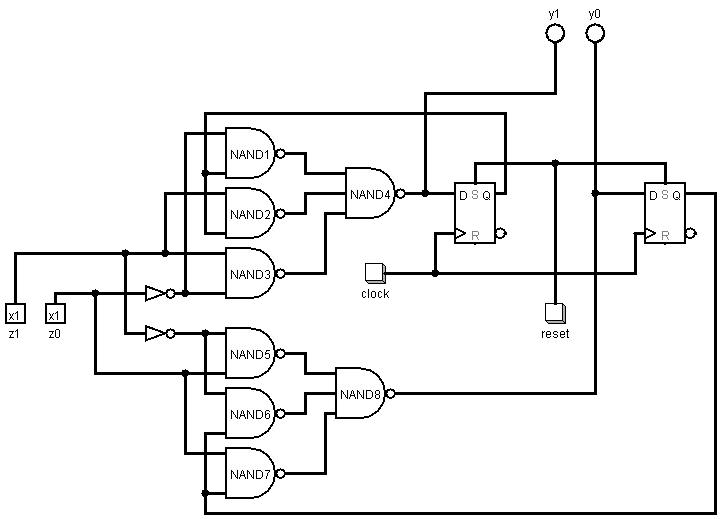
\includegraphics[width=\paperwidth - 30mm]{schem/circuitv2.png}}
			Schemat 1
		\end{center}

	\section{Wnioski/podsumowanie}
	
			W celu sprawdzenia poprawności działania należało przeprowadzić testy dla wszystkich możliwych kombinacji wejść. Pierwsze ćwiczenie zostało wykonane poprawnie, natomiast drugie ćwiczenie zostało zaprojektowane bez pomocy tabeli prawdy, przez co uruchomienie układu się nie powiodło. Poprawny model układu został umieszczony w sprawozdaniu.
	
\end{document}